\documentclass[journal,12pt,twocolumn]{IEEEtran}

\usepackage{setspace}
\usepackage{gensymb}
\singlespacing
\usepackage[cmex10]{amsmath}

\usepackage{amsthm}
\usepackage{amsmath,amssymb}
\usepackage{mathrsfs}
\usepackage{txfonts}
\usepackage{stfloats}
\usepackage{bm}
\usepackage{cite}
\usepackage{cases}
\usepackage{subfig}

\usepackage{longtable}
\usepackage{multirow}
\usepackage{float}
\usepackage{enumitem}
\usepackage{mathtools}
\usepackage{steinmetz}
\usepackage{tikz}
\usepackage{circuitikz}
\usepackage{verbatim}
%\usepackage{tfrupee}
\usepackage[breaklinks=true]{hyperref}
\usepackage{graphicx}
\usepackage{tkz-euclide}
\usepackage{stackengine}
\usetikzlibrary{calc,math}
\usepackage{listings}
    \usepackage{color}                                            %%
    \usepackage{array}                                            %%
    \usepackage{longtable}                                        %%
    \usepackage{calc}                                             %%
    \usepackage{multirow}                                         %%
    \usepackage{hhline}                                           %%
    \usepackage{ifthen}                                           %%
    \usepackage{lscape}     
\usepackage{multicol}
\usepackage{chngcntr}
\usepackage{bm}
\DeclareMathOperator*{\Res}{Res}

\renewcommand\thesection{\arabic{section}}
\renewcommand\thesubsection{\thesection.\arabic{subsection}}
\renewcommand\thesubsubsection{\thesubsection.\arabic{subsubsection}}

\renewcommand\thesectiondis{\arabic{section}}
\renewcommand\thesubsectiondis{\thesectiondis.\arabic{subsection}}
\renewcommand\thesubsubsectiondis{\thesubsectiondis.\arabic{subsubsection}}
\providecommand{\laplace}{\overset{\mathcal{L}}{ \rightleftharpoons}}
\providecommand{\abs}[1]{\left\vert#1\right\vert}
\providecommand{\z}{\overset{z}{ \rightleftharpoons}}
\hyphenation{op-tical net-works semi-conduc-tor}
\def\inputGnumericTable{}                                 %%

\lstset{
%language=C,
frame=single, 
breaklines=true,
columns=fullflexible
}
\makeatletter
\setlength{\@fptop}{0pt}
\makeatother
\begin{document}

\newtheorem{theorem}{Theorem}[section]
\newtheorem{problem}{Problem}
\newtheorem{proposition}{Proposition}[section]
\newtheorem{lemma}{Lemma}[section]
\newtheorem{corollary}[theorem]{Corollary}
\newtheorem{example}{Example}[section]
\newtheorem{definition}[problem]{Definition}

\newcommand{\BEQA}{\begin{eqnarray}}
\newcommand{\EEQA}{\end{eqnarray}}
\newcommand{\define}{\stackrel{\triangle}{=}}
\bibliographystyle{IEEEtran}
\raggedbottom
\setlength{\parindent}{0pt}
\providecommand{\mbf}{\mathbf}
\providecommand{\pr}[1]{\ensuremath{\Pr\left(#1\right)}}
\providecommand{\qfunc}[1]{\ensuremath{Q\left(#1\right)}}
\providecommand{\sbrak}[1]{\ensuremath{{}\left[#1\right]}}
\providecommand{\lsbrak}[1]{\ensuremath{{}\left[#1\right.}}
\providecommand{\rsbrak}[1]{\ensuremath{{}\left.#1\right]}}
\providecommand{\brak}[1]{\ensuremath{\left(#1\right)}}
\providecommand{\lbrak}[1]{\ensuremath{\left(#1\right.}}
\providecommand{\rbrak}[1]{\ensuremath{\left.#1\right)}}
\providecommand{\cbrak}[1]{\ensuremath{\left\{#1\right\}}}
\providecommand{\lcbrak}[1]{\ensuremath{\left\{#1\right.}}
\providecommand{\rcbrak}[1]{\ensuremath{\left.#1\right\}}}
\DeclarePairedDelimiter\ceil{\lceil}{\rceil}
\DeclarePairedDelimiter\floor{\lfloor}{\rfloor}
\theoremstyle{remark}
\newtheorem{rem}{Remark}
\newcommand{\sgn}{\mathop{\mathrm{sgn}}}
\providecommand{\abs}[1]{\vert#1\vert}
\providecommand{\res}[1]{\Res\displaylimits_{#1}} 
\providecommand{\norm}[1]{\lVert#1\rVert}
%\providecommand{\norm}[1]{\lVert#1\rVert}
\providecommand{\mtx}[1]{\mathbf{#1}}
\providecommand{\mean}[1]{E[ #1 ]}
\providecommand{\fourier}{\overset{\mathcal{F}}{ \rightleftharpoons}}
%\providecommand{\hilbert}{\overset{\mathcal{H}}{ \rightleftharpoons}}
\providecommand{\system}{\overset{\mathcal{H}}{ \longleftrightarrow}}
	%\newcommand{\solution}[2]{\textbf{Solution:}{#1}}
\newcommand{\solution}{\noindent \textbf{Solution: }}
\newcommand{\cosec}{\,\text{cosec}\,}
\newcommand*{\permcomb}[4][0mu]{{{}^{#3}\mkern#1#2_{#4}}}
\newcommand*{\perm}[1][-3mu]{\permcomb[#1]{P}}
\newcommand*{\comb}[1][-1mu]{\permcomb[#1]{C}}
\newcommand\xrowht[2][0]{\addstackgap[.5\dimexpr#2\relax]{\vphantom{#1}}}
\providecommand{\dec}[2]{\ensuremath{\overset{#1}{\underset{#2}{\gtrless}}}}
\newcommand{\myvec}[1]{\ensuremath{\begin{pmatrix}#1\end{pmatrix}}}
\newcommand{\mydet}[1]{\ensuremath{\begin{vmatrix}#1\end{vmatrix}}}
\numberwithin{equation}{subsection}
\makeatletter
\@addtoreset{figure}{problem}
\makeatother
\let\StandardTheFigure\thefigure
\let\vec\mathbf
\renewcommand{\thefigure}{\theproblem}
\def\putbox#1#2#3{\makebox[0in][l]{\makebox[#1][l]{}\raisebox{\baselineskip}[0in][0in]{\raisebox{#2}[0in][0in]{#3}}}}
     \def\rightbox#1{\makebox[0in][r]{#1}}
     \def\centbox#1{\makebox[0in]{#1}}
     \def\topbox#1{\raisebox{-\baselineskip}[0in][0in]{#1}}
     \def\midbox#1{\raisebox{-0.5\baselineskip}[0in][0in]{#1}}
\vspace{3cm}
\title{Exam-2}
\author{Chirag Mehta - AI20BTECH11006}
\maketitle
\newpage
\bigskip
\renewcommand{\thefigure}{\theenumi}
\renewcommand{\thetable}{\theenumi}
Download all the python codes from
\begin{lstlisting}
https://github.com/cmaspi/EE3900/tree/main/exam-2/Codes
\end{lstlisting}
latex-tikz codes from 
\begin{lstlisting}
https://github.com/cmaspi/EE3900/blob/main/exam-2/main.tex
\end{lstlisting}
\section{Problem}
(Q 3.1 a,b,c) 
Determine the $z-$transform, including the region of convergence, for each of the following sequences
\begin{enumerate} [label= (\alph*)]
    \item $\brak{\frac{1}{2}}^n u[n]$
    \item $-\brak{\frac{1}{2}}^n u[-n-1]$
    \item $\brak{\frac{1}{2}}^n u[-n]$
\end{enumerate}

\section{Solution}
\begin{definition}\label{def:z}
    The $z$ tansform of a function is defined as
    \begin{align}
        x[n] &\z X(z)\\
        X(z) &=\sum_{n=-\infty}^{\infty} x[n]z^{-n}
    \end{align}
\end{definition}
\begin{definition}\label{def:u_n}
    The $u[n]$ function is defined as
    \begin{align}
        u[n] = 
        \begin{cases}
        1 & n\geq0\\
        0 & otherwise
        \end{cases}
    \end{align}
\end{definition}
\begin{enumerate}[label= (\alph*)]
    \item $\brak{\frac{1}{2}}^n u[n]$
    \begin{align}
        x[n]=\brak{\frac{1}{2}}^n u[n]
    \end{align}
    Using~\eqref{def:z} and~\eqref{def:u_n}
    \begin{align}
        X(z)&=\sum_{n=-\infty}^{\infty} \brak{\frac{1}{2}}^n u[n]z^{-n}\\
        &=\sum_{n=0}^{\infty} \brak{\frac{z^{-1}}{2}}^n\\
        &=\frac{1}{1-\frac{1}{2}z^{-1}},\, ROC=\abs{\frac{z^{-1}}{2}} < 1\\
        &=\frac{2}{2-z^{-1}},\, ROC=\abs{z}>\frac{1}{2}
    \end{align}
    \begin{figure}[!ht]
        \centering
        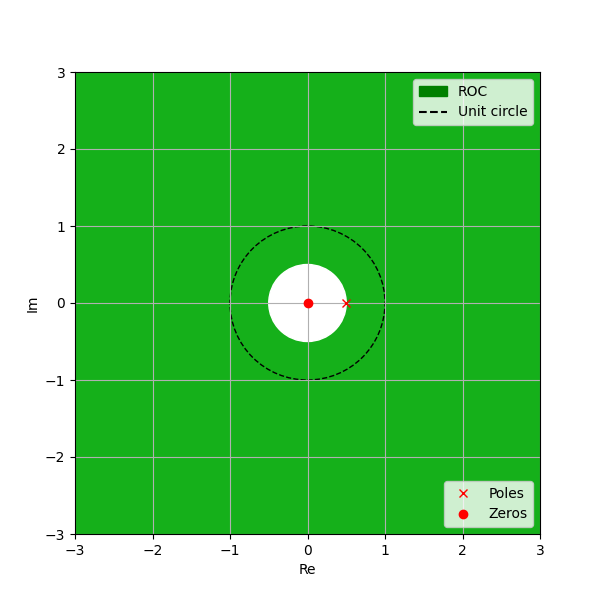
\includegraphics[width=\columnwidth]{plot/a}
        \caption{Pole-zero plot of the system}
        \label{a}
    \end{figure}

    \item $-\brak{\frac{1}{2}}^n u[-n-1]$
    \begin{align}
        x[n]=-\brak{\frac{1}{2}}^n u[-n-1]
    \end{align}
    Using~\eqref{def:z} and~\eqref{def:u_n}
    \begin{align}
        X(z)&=\sum_{n=-\infty}^{\infty} -\brak{\frac{1}{2}}^n u[-n-1]\\
        &=\sum_{n=-\infty}^{-1} -\brak{\frac{1}{2}}^n z^{-n}\\
        &=-\sum_{n=1}^{\infty} \brak{2z}^n\\
        &=\frac{-2z}{1-2z},\, ROC=\abs{2z} < 1\\
        &=\frac{2}{2-z^{-1}},\, ROC=\abs{z}<\frac{1}{2}
    \end{align}
    \begin{figure}[!ht]
        \centering
        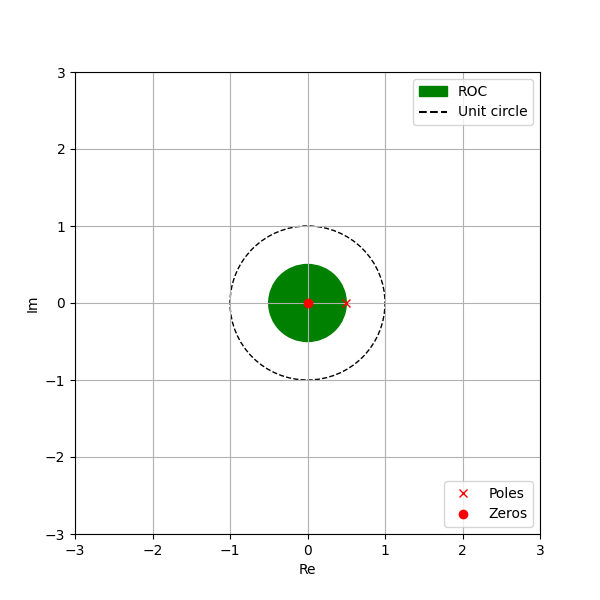
\includegraphics[width=\columnwidth]{plot/b}
        \caption{Pole-zero plot of the system}
        \label{b}
    \end{figure}


    \item $\brak{\frac{1}{2}}^n u[-n]$
    \begin{align}
        x[n]=\brak{\frac{1}{2}}^n u[-n]
    \end{align}
    Using~\eqref{def:z} and~\eqref{def:u_n}
    \begin{align}
        X(z)&=\sum_{n=-\infty}^{\infty} \brak{\frac{1}{2}}^n u[-n]z^{-n}\\
        &=\sum_{n=-\infty}^{0} \brak{\frac{1}{2z}}^n \\
        &=\sum_{n=0}^{\infty} \brak{2z}^n\\
        &=\frac{1}{1-2z},\, ROC=\abs{2z} < 1\\
        &=\frac{1}{1-2z},\, ROC=\abs{z}<\frac{1}{2}
    \end{align}
    \begin{figure}[!ht]
        \centering
        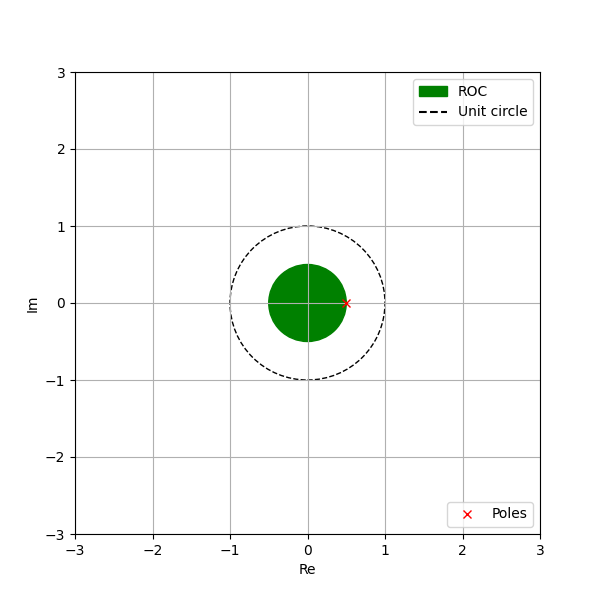
\includegraphics[width=\columnwidth]{plot/c}
        \caption{Pole-zero plot of the system}
        \label{c}
    \end{figure}
\end{enumerate}
    
\end{document}